\mychapter{State Estimation}{State Estimation}{}
\label{chap:stateestimation}

\mysection{Introduction}{Introduction}
\label{sec:stateintro}

\mysection{Recursive Estimation}{Recursive Estimation}
\label{sec:stateEKF}

This section describes the element of recrusive estimators along with a few commonly-used estimators in the fields of localisation and tracking. A recursive estimoter uses the previous
distrubution over a set of systm states and curent sensor data to estimte the current state distribution. Figure 3.1 illustrates the basic workings of a discrete recursive filter.

\begin{figure}[H]
    \centering
    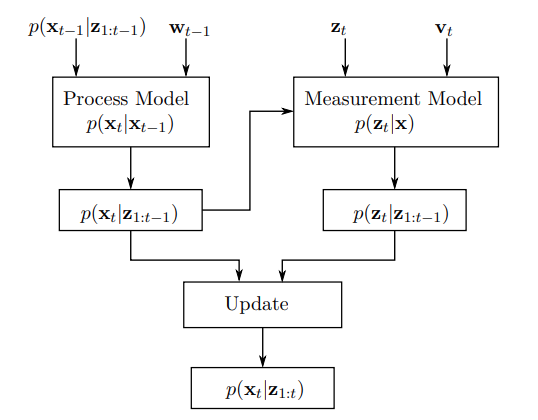
\includegraphics[width=0.5\linewidth]{figures/StateEstimation/Recursive Estimation.png}
    \caption{Recursive estimator algorithm flowchart}
    \label{}
\end{figure}

The state vector is represented by $\mathbf{x}_t$ for the estimation problem in the discrete time domain. The process, or the state transition function, is expressed As
\begin{equation}
    \mathbf{x}_t = \mathbf{f}(\mathbf{x}_{t-1},\mathbf{u}_{t-1},\mathbf{w}_{t-1})
\end{equation}

where $\mathbf{f}$ is either a linear or non-linear transtion fucntion and $\mathbf{w}_t$ represents the process noise. New observation data, $\mathbf{z}_t$, is available at
discrete timesteps and can be related to $\mathbf{x}_t$ by the measurement function,

\begin{equation}
    \mathbf{z}_t = \mathbf{h}(\mathbf{x}_t,\mathbf{v}_t)
\end{equation}

The measurement uncertainty is represented by $\mathbf{v}_t$ and $\mathbf{h}$ is the observation model, which can also either be linear or non-linear. The goal is to obtain the
posterior distribution, $p(\mathbf{x}|\mathbf{z}_{1:t})$, over the state vector $\mathbf{x}_t$. This is done by recursively performing the process and measurement updates.

At a time $t$, the posterior distribution over $\mathbf{x}_{t-1}$ at time $t-1$ is known and the prior distribution at t is calcualted As

\begin{equation}
    p(\mathbf{x}_t|\mathbf{z}_{1:t-1}) = \int p(\mathbf{x}_t|\mathbf{x}_{t-1})p(\mathbf{x}_{t-1}|\mathbf{z}_{1:t-1})\ d\mathbf{x}_{t-1}
\end{equation}

The measruement update is used to calculate the new posterior, at time $t$ , given the prior state distribution according to Bayes' rule,

\begin{equation}
    p(\mathbf{x}_t|\mathbf{z}_{1:t}) = 
    \frac{p(\mathbf{z}_t|\mathbf{x}_t)p(\mathbf{x}_t|\mathbf{z}_{1:t-1})}{p(\mathbf{z}_t|\mathbf{z}_{1:t-1})}
\end{equation}

The Kalman filter is a popular estimator used in pose estimation porblems. It is a special case of the Bayes filter, where the Guassian noise distributions are assumed.
The assumption is also made that the initial distibution of the system can be represented by a Gaussian distribution. A control and measurement update is executed
at each sampling instant to update the distibutionover the states. If the previous state distribution is Gaussian, then the updated current distribution will also be Gaussian
and therefore the best estimate is chosen as the mean of the distribution.

Differen variants of the Kalman Filter exists, of which the extended and unscented Kalman Filter are the most popular, eah with their own unique characteristics.

The extended Kalman Filter (EKF) overcomes the restrictions of the linear filter by approximating non-linear functions to be linear using a first-order Taylor expansion.
The mean position of the state vector is used as the linearisation point around which the tangent of the non-linear function is calcualted, allowing the use of standard
Kalman Filter equations. It is typically more efficient than other non-linear filters which sometimes comes at a cost or reduced accuracy.

The unscented Kalman Filter (UKF) uses stochiatic linearisation to deal with non-linear systems. Given a distribution with a known mean and covariance, a set of weighted points,
known as sigma points, are chosen and transformed using the non-linear function. A new distribution is determined from the transformed sigma points. The process and observation
functions do not need to be differentiable and the output is based on vlaues in a larger region, rather than a local approximation.

\mysection{Kalman Filter}{Kalman Filter}


Kalman filters are well suited for localistation problems since the nature of these systems are normally non-linear. Both the linear and non-linear variants of the Kalman Filter
are concenerd with estimating states using motion model to perform this data fusion. The following equations are used to model the system.

\begin{equation}
    \mathbf{x}_t = A_t\mathbf{x}_{t-1} + B\mathbf{u}_{t-1} + \mathbf{\epsilon}
    \mathbf{z}_t = C_t\mathbf{x}_t + \mathbf{\zeta}
\end{equation}

where

\begin{equation}
    \epsilon = \mathcal{N}(\mathbf{0};R)
    \zeta = \mathcal{N}(\mathbf{0};Q)
\end{equation}

The matrices R and Q are the known covarianve matrices of the process and observation noise, repsectivly and the matrices A, B and C form part of the linear functions.

These equations can be used to calculate the posterior distrobution

\begin{equation}
    p(\mathbf{y}_t|\mathbf{u}_{1:t},\mathbf{z}_{1:t}) = \mathcal{N}(\mu_t ;\Sigma_t)
\end{equation}

The state estimation problem in this project makes use of non-linear system models, and a high-dimensinal state space. The EKF is well suited for this problem, since it
accomodates non-linear process and observation models and is capable of dealing with high-dimensional state spaces. The EKF os often use for the SLAM problem and is well
known in the field of robotics and localisation.

The rigid body motion models and measurements models of systems are, however, non-linear. Therefore, a general non-linear description is used for the motion and measurement models

\begin{equation}
    \mathbf{y}_t = \mathbf{g}(\mathbf{y}_{t-1},\mathbf{u}_t) + \boldsymbol{\epsilon}
\end{equation}

\begin{equation}
    \mathbf{z}_t = \mathbf{h}(\mathbf{y}_t) + \boldsymbol{\zeta}     
\end{equation}

The motion and measurement functions, $\mathbf{g}$ and $\mathbf{h}$, are non-linear vector functions.  These are linearised to enable the use of the Kalman filter equations. 
The non-linear vector functions, $\mathbf{f}(\mathbf{x}) = [f_1(\mathbf{x}),f_2(\mathbf{x}),...,f_m(\mathbf{x})]^T$, is linearised around its mean value, $\mu$, using
a Taylor series expansion.

\begin{equation}
    \mathbf{f}(\mathbf{x}) \approx \mathbf{f}(\boldsymbol{\mu}) + \mathbf{f}'(\boldsymbol{\mu})(\mathbf{x}-\boldsymbol{\mu})
\end{equation}

where


\begin{equation}
  \begin{aligned}
    \mathbf{f}'(\mathbf{x})
      &= \mathit{F}(\mathbf{x})
       = \frac{\partial \mathbf{f}(\mathbf{x})}{\partial \mathbf{x}} \\
      &=
    \begin{bmatrix}
      \dfrac{\partial f_1}{\partial x_1} & \cdots & \dfrac{\partial f_1}{\partial x_n} \\
      \vdots & \ddots & \vdots \\
      \dfrac{\partial f_m}{\partial x_1} & \cdots & \dfrac{\partial f_m}{\partial x_n}
    \end{bmatrix}_{m \times n}
  \end{aligned}
\end{equation}

$\mathit{F}(\mathbf{x})$ is referred to as the Jacobian matrix. Using this linearisation, the vector function, $\mathbf{g}$ and $\mathbf{h}$
are approximated as,

\begin{equation}
    \mathbf{y}_{t-1}, \mathbf{u}_t \approx \mathbf{g}(\boldsymbol{\mu}_{t-1}, \mathbf{u}_t) + \mathbf{G}_t (\mathbf{y}_{t-1} - \boldsymbol{\mu}_{t-1})
\end{equation}

\begin{equation}
    \mathbf{h}(\mathbf{y}_t) \approx \mathbf{h}(\boldsymbol{\mu}_t) + \mathbf{H}_t (\mathbf{y}_t - \boldsymbol{\mu}_t)
\end{equation}

where \( \mathbf{G}_t \) and \( \mathbf{H}_t \) are the Jacobian matrices of \( \mathbf{g} \) and \( \mathbf{h} \), respectively. This linearisation leads to the approximate distribution

\begin{equation}
    p(\mathbf{y}_t \mid \mathbf{u}_{1:t}, \mathbf{z}_{1:t}) \approx \mathcal{N}(\boldsymbol{\mu}_{t \mid t}, \boldsymbol{\Sigma}_{t \mid t})
\end{equation}



\mysection{System Modelling}{System Modelling}
\label{sec:statesystemmodel}

\begin{figure}[htbp]
    \centering
    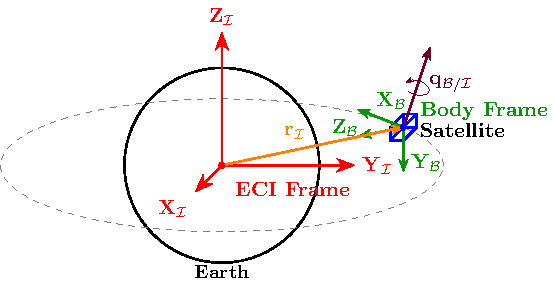
\includegraphics[width=0.8\textwidth]{figures/Figure1.pdf}
    \caption{Satellite pose estimation concept showing orbital geometry, reference frames}
    \label{fig:System Modelling}
\end{figure}

As we can see in Figure \ref{fig:System Modelling} to determine the pose of the satellite the position and the attitude of the satellite in the ECI reference frames needs to be
determines

\begin{equation}
    \mathbf{x}_t =
    \begin{bmatrix}
        \mathbf{r}_\mathcal{I} & \mathbf{v}_\mathcal{I} & \mathbf{q}_\mathcal{B/I} & \boldsymbol{\omega}_\mathcal{B/I}^\mathcal{B}
    \end{bmatrix}
    ^T
\end{equation}

\mysubsection{Motion Model}{Motion Model}
\label{sec:statemotionmodel}

The rotation of the satellite body is non-linear and the satellite motion from one timestep to the next when using Newton-Eular coupling can be described by the vector function
$\mathbf{g}$,

\begin{equation}
    \mathbf{x}_t = \mathbf{g}(\mathbf{x}_{t-1},\mathbf{u}_t) + \boldsymbol{\epsilon}
\end{equation}

which is expanded to,

\begin{equation}
    \mathbf{x}_t
    =
    \begin{bmatrix}
        r_{x,t} \\
        r_{y,t} \\
        r_{z,t} \\
        v_{x,t} \\
        v_{y,t} \\
        v_{z,t} \\
        q_{s,t} \\
        q_{x,t} \\
        q_{y,t} \\
        q_{z,t} \\
        \omega_{x,t} \\
        \omega_{y,t} \\
        \omega_{z,t} \\
    \end{bmatrix}
    = \mathbf{x}_{t-1} +
    \begin{bmatrix}
        v_{x,t-1} \\
        v_{x,t-1} \\
        v_{x,t-1} \\
        -\frac{\mu}{|\mathbf{r}|^3}*r_{x,t-1} + J2_{x,t-1} \\
        -\frac{\mu}{|\mathbf{r}|^3}*r_{y,t-1} + J2_{y,t-1} \\
        -\frac{\mu}{|\mathbf{r}|^3}*r_{z,t-1} + J2_{z,t-1} \\
        \frac{1}{2}(-\omega_{x,t-1}q_{x,t-1} - \omega_{y,t-1}q_{y,t-1} - \omega_{z,t-1}q_{z,t-1}) \\
        \frac{1}{2}( \omega_{x,t-1}q_{s,t-1} + \omega_{z,t-1}q_{y,t-1} - \omega_{y,t-1}q_{z,t-1}) \\
        \frac{1}{2}( \omega_{y,t-1}q_{s,t-1} - \omega_{z,t-1}q_{x,t-1} + \omega_{x,t-1}q_{z,t-1}) \\
        \frac{1}{2}( \omega_{z,t-1}q_{s,t-1} + \omega_{y,t-1}q_{x,t-1} - \omega_{x,t-1}q_{y,t-1}) \\
        \frac{1}{\mathit{I}_{xx}}(\mathit{I}_{yy}-\mathit{I}_{zz})\omega_{y,t-1}\omega_{z,t-1} \\
        \frac{1}{\mathit{I}_{yy}}(\mathit{I}_{zz}-\mathit{I}_{xx})\omega_{z,t-1}\omega_{x,t-1} \\
        \frac{1}{\mathit{I}_{zz}}(\mathit{I}_{xx}-\mathit{I}_{yy})\omega_{x,t-1}\omega_{y,t-1}
    \end{bmatrix}
    \Delta t + 
    \begin{bmatrix}
        0 \\
        0 \\
        0 \\
        0 \\
        0 \\
        0 \\
        0 \\
        0 \\
        0 \\
        0 \\
        \mathit{T}_x/\mathit{I}_x \\
        \mathit{T}_y/\mathit{I}_y \\
        \mathit{T}_z/\mathit{I}_z
    \end{bmatrix}
\end{equation}

The body-fixed axes of the target are chosen to coincide with its principle axes of inertia. The principle moment of inertia are given barycenter

\begin{equation}
    \mathbf{I}_\mathcal{B} = 
    \begin{bmatrix}
        \mathit{I}_{xx} & 0 & 0 \\
        0 & \mathit{I}_{yy} & 0 \\
        0 & 0 & \mathit{I}_{zz}
    \end{bmatrix}
\end{equation}

External torques, $\mathit{T}_x$, $\mathit{T}_y$ and $\mathit{T}_z$, are asssumed to be zero and there is thus no control input, $\mathbf{u}_t$. 

Thus 

\begin{equation}
    \mathbf{x}_t = \mathbf{g}(\mathbf{x}_{t-1})
\end{equation}

where

\begin{equation}
    \mathbf{x}_t
    =
    \begin{bmatrix}
        r_{x,t} \\
        r_{y,t} \\
        r_{z,t} \\
        v_{x,t} \\
        v_{y,t} \\
        v_{z,t} \\
        q_{s,t} \\
        q_{x,t} \\
        q_{y,t} \\
        q_{z,t} \\
        \omega_{x,t} \\
        \omega_{y,t} \\
        \omega_{z,t} \\
    \end{bmatrix}
    = \mathbf{x}_{t-1} +
    \begin{bmatrix}
        v_{x,t-1} \\
        v_{x,t-1} \\
        v_{x,t-1} \\
        -\frac{\mu}{|\mathbf{r}|^3}*r_{x,t-1} + J2_{x,t-1} \\
        -\frac{\mu}{|\mathbf{r}|^3}*r_{y,t-1} + J2_{y,t-1} \\
        -\frac{\mu}{|\mathbf{r}|^3}*r_{z,t-1} + J2_{z,t-1} \\
        \frac{1}{2}(-\omega_{x,t-1}q_{x,t-1} - \omega_{y,t-1}q_{y,t-1} - \omega_{z,t-1}q_{z,t-1}) \\
        \frac{1}{2}( \omega_{x,t-1}q_{s,t-1} + \omega_{z,t-1}q_{y,t-1} - \omega_{y,t-1}q_{z,t-1}) \\
        \frac{1}{2}( \omega_{y,t-1}q_{s,t-1} - \omega_{z,t-1}q_{x,t-1} + \omega_{x,t-1}q_{z,t-1}) \\
        \frac{1}{2}( \omega_{z,t-1}q_{s,t-1} + \omega_{y,t-1}q_{x,t-1} - \omega_{x,t-1}q_{y,t-1}) \\
        \frac{1}{\mathit{I}_{xx}}(\mathit{I}_{yy}-\mathit{I}_{zz})\omega_{y,t-1}\omega_{z,t-1} \\
        \frac{1}{\mathit{I}_{yy}}(\mathit{I}_{zz}-\mathit{I}_{xx})\omega_{z,t-1}\omega_{x,t-1} \\
        \frac{1}{\mathit{I}_{zz}}(\mathit{I}_{xx}-\mathit{I}_{yy})\omega_{x,t-1}\omega_{y,t-1}
    \end{bmatrix}
    \Delta t
\end{equation}

\mysubsection{Measurement Model}{Measurement Model}
\label{sec:statemeasuremtmodel}

\mysubsection{Earth Tracker Measurement Model}{Earth Tracker Measurement Model}

The Earth Tracker sends 2 inputs to the EKF, the measurement of the Earth tracker itself 

\begin{equation}
    \mathbf{z}_{ET} = \mathbf{f}_\mathcal{B} =
    \begin{bmatrix}
        x_\mathcal{B} \\
        y_\mathcal{B} \\
        z_\mathcal{B}
    \end{bmatrix}
\end{equation}

And the Geolocated feature vector through feature mathcing also refered to as the catalogue vector. $ \mathbf{f}_\mathcal{R}$

To transform this vector into a vector to be comparable to the measurement.

\begin{equation}
    \mathbf{f}_\mathcal{B} = \mathbf{A}_{\mathcal{I},t}^\mathcal{B} \times \mathbf{A}_{\mathcal{R},t}^\mathcal{I} \times \mathbf{f}_\mathcal{R}
\end{equation}


Where $\mathbf{A}_{\mathcal{O},t}^\mathcal{B}$ is a function of the the quaternion $\mathbf{q}_\mathcal{B/I}$





\mysubsection{Other Sensor Measurment model}{Other Sensor Measruement Models}

\textbf{GPS}

For the GPS it measures position in the ECEF reference frame, so it need to be converted to toe ECI reference frame.

\begin{equation}
    \mathbf{H}_{GPS} = 
    \begin{bmatrix}
        \cos(\omega_et) & -\sin(\omega_et) & 0 & \mathbf{0}_{1\times10} \\
        \sin(\omega_et) & \cos(\omega_et) & 0 & \mathbf{0}_{1\times10} \\
        0 & 0 & 1 & \mathbf{0}_{1\times10}
    \end{bmatrix}
\end{equation}

\textbf{Gyroscope}

for the gyroscope, the gyroscope alreadu measures $\boldsymbol{\omega}^\mathcal{B}_\mathcal{B/I}$ so it is just a direct relationship.

\begin{equation}
    \mathbf{H}_{GYR} = 
    \begin{bmatrix}
        \mathbf{0}_{1\times10} & 1 & 0 & 0 \\
        \mathbf{0}_{1\times10} & 0 & 1 & 0 \\
        \mathbf{0}_{1\times10} & 0 & 0 & 1 
    \end{bmatrix}
\end{equation}

\textbf{TRIAD and Star Tracker}

The Coarse Sun Sensor and Magnetometer measurements are pre-processed into an attitue value of the body frame relative to the Inertial reference frame.$\mathbf{q}_\mathcal{B/I}$

\begin{equation}
    \mathbf{H}_{TRIAD} = 
    \begin{bmatrix}
        \mathbf{0}_{1\times6} & 1 & 0 & 0 & 0 & \mathbf{0}_{1\times3}\\
        \mathbf{0}_{1\times6} & 0 & 1 & 0 & 0 &\mathbf{0}_{1\times3}\\
        \mathbf{0}_{1\times6} & 0 & 0 & 1 & 0 &\mathbf{0}_{1\times3}\\
        \mathbf{0}_{1\times6} & 0 & 0 & 0 & 1 & \mathbf{0}_{1\times3}
    \end{bmatrix}
\end{equation}

\mysection{Conclusion}{Conclusion}
\label{sec:stateconclusion}